\chapter{Asking Billionaires How They Got Rich! (Beverly Hills)}

These notes follow the School of Hard Knocks interview on Beverly Hills, curated in this volume by LazyingArt LLC. The lecture does not proceed as a blackboard derivation. Its mathematics is buried in the order of the questions themselves: starting below zero, paying lenders before oneself, listening before pricing, noticing tiny details, distinguishing firm revenue from owner extraction, and separating a small market from a large one. No validated mathematical frame survives for this lecture, so every formula below is a cautious reconstruction from the spoken sequence itself.

\section{Cold Open and Rodeo Drive Reset}

Before anything is explained, the lecture throws a cluster of later outcomes at us: billionaire status, a sold company, a teenage wealth claim, very large annual sales, and a hard line about schooling. We should not read that cold open as a stable ledger. Its function is to spend surprise first and explanation later.

The real beginning comes with the reset in Beverly Hills. There the host tells us what kind of inquiry we are in: not sightseeing, but a search for mechanisms. Rodeo Drive is treated as a testing ground for a set of transferable questions. How was wealth created? How large did it become? By what habits, structures, or relations was it preserved? The rest of the lecture unfolds as a sequence of local answers to those questions.

\section{Busboy to Boardroom: Negative Capital, Sale Scale, and Debt Order}

The first full case is the hospitality operator. The narrative quickly moves from biography into arithmetic: busboy to boardroom, Diamond Resorts, Hilton, hotels in many countries, and then the shock of beginning below zero. The two clean numbers that anchor the case are
\begin{equation}
W_0 = -\$20\,\text{million}, \qquad N_{\text{countries}} = 35.
\end{equation}
This is the lecture's first serious quantitative move. Wealth is not being narrated as the accumulation of surplus from a secure baseline. It begins in deficit.

The same speaker then gives two valuation figures. The transcript is noisy, so we keep them without overcommitting the labels:
\begin{equation}
V_1 \approx \$2.2\,\text{billion}, \qquad V_2 \approx \$3.3\,\text{billion}.
\end{equation}
What matters is not the exact bookkeeping category but the scale. The lecture wants us to feel the jump from a negative starting condition to a business measured in billions.

The transition from life story to commercial method comes through debt discipline. The speaker's point is not that debt is absent, but that the order of obligations is never forgotten. In the cleanest notation available to us,
\begin{equation}
\text{Pay(partners)},\ \text{Pay(banks)} \prec \text{Pay(owner)}.
\end{equation}
This is not a formal waterfall. It is a rule of conduct: owner payout is residual, and trust with counterparties is primary.

\subsection{Question \& Answer}

Question: why does the lecture make listening the real sales mechanism rather than persuasion alone?

Answer: because the speaker is asked, in effect, whether it can really be that simple, and he answers by reducing selling to information before pressure. The single word \emph{listen} is then unpacked: customers, friends, and bankers reveal the pathway. We may therefore write
\begin{equation}
\mathrm{listen} \Rightarrow \text{pathway to sale}.
\end{equation}
The point is not passivity. Listening tells us what the counterparty will count as real value. Only then does the second line have content:
\begin{equation}
V_{\text{delivered}} \ge P_{\text{asked}}.
\end{equation}
If we do not know what the other side values, we do not yet know what we are pricing. The lecture's order is therefore exact: first listen, then deliver, then ask.

\section{Negotiation Silence, Banks, Shocks, and Human Environment}

The hospitality interview does not stop with sales. It immediately pushes outward into negotiation, banking relations, macro shock, and social placement. Negotiation is reduced to a sharp field rule:
\begin{equation}
\mathrm{speak\ first\ in\ ripe\ deal} \Rightarrow \text{weaker bargaining position}.
\end{equation}
This is not game theory in the formal sense. It is an operator's heuristic: once a deal is ready, unnecessary speech leaks advantage.

The lecture then makes what at first seems like an unrelated move. The speaker says he never negotiated aggressively with his banks; he preferred that his banks make money with him. We should not universalize this into a theorem about optimal financing. The narrower point is that the bank relationship is treated as repeated rather than one-shot. The speaker wants continuity of support, not merely the best isolated rate.

From there the lecture widens still further, from counterparties to exogenous shock. The example is 9/11. Flights stop. Hotel guests disappear. Revenue vanishes. In notation,
\begin{equation}
R_{\text{hotel}} \to 0 \qquad \text{after the flight-stoppage shock.}
\end{equation}
This is one of the cleanest causal reductions in the chapter. Nothing here depends on the quality of the product or the charm of the seller. The business is suddenly exposed to a change in the outer world.

\subsection{Question \& Answer}

Question: why does the lecture place silence in negotiation, generosity toward banks, and crisis survival inside one commercial worldview?

Answer: because in all three cases the speaker is thinking about endurance rather than isolated victory. The logic can be read in three steps:
\begin{enumerate}
\item In negotiation, we preserve informational advantage by not speaking too soon.
\item In financing, we preserve relational capital by keeping banks and investors willing to remain in the game.
\item In crisis, we discover whether those preserved relations and prior disciplines are enough to carry the business through an external blow.
\end{enumerate}
So the worldview is ecological rather than merely tactical. We are not just learning how to win a deal. We are learning how to stay legible and survivable inside a network of counterparties and shocks.

The interview then pushes the same ecological logic into the human environment. One must stay out of the ``bad zip code,'' meaning bad people, and one must distrust luxuries that are only rented symbols of success. The point is not prudery. It is that business method is inseparable from the people around whom one lives and the signals one chooses to emit.

The host's recap after this interview is not filler. He takes the word \emph{listen} and translates it into customer feedback, product adjustment, and market share. That translation prepares the next case.

\section{Operational Detail: The Salon Founder on Feedback and Fit}

The salon founder does not overturn the first billionaire's doctrine; she gives it finer resolution. The story begins with no money, then introduces a brother who had made some money at Yahoo, then a sweat-equity arrangement, then substantial fundraising, and finally a sale. The stable quantitative cluster is
\begin{equation}
S_{\text{salon}} = \$155\,\text{million}, \qquad E_{\text{operator}} = 50\%, \qquad C_{\text{raised}} \approx \$75\,\text{million}.
\end{equation}
We keep the direct sale figure, \(\$155\) million, rather than the host's later inflated restatement.

The host then introduces a failure-rate heuristic:
\begin{equation}
p_{\text{fail},5\text{yr}} \approx \frac{8}{10}.
\end{equation}
This should not be treated as an audited statistic. Its function in the lecture is motivational: it sets up the question of why so many firms die.

\subsection{Question \& Answer}

Question: why do tiny environmental details become business-killing variables?

Answer: because the lecture treats customer experience as a chain of small frictions and small reassurances. The salon founder's answer can be written compactly as
\begin{equation}
\text{feedback ignored} \Rightarrow \text{fit deteriorates} \Rightarrow \text{customer exit}.
\end{equation}
The transcript then spells out what this means operationally: the bathroom is clean or not; the person at the front desk has attitude or not; the chair scrapes loudly or not; the room feels cared for or not. None of these looks decisive in isolation. Together they create the hidden state that the customer feels before the customer can fully articulate it.

This interview then makes a second move. The speaker turns from customer fit to investor fit. Raising money is not enough. One must raise it from people whose time horizon, vision, and desired form of the company are aligned with the founder's own. The lecture's metaphor is exact: capital is a marriage, not merely a check.

\section{The Interrupted Middle: Mentorship as Host Doctrine}

At this point the lecture deliberately interrupts itself. The School of Mentors segment is structurally real, but it is not another interview-derived theorem. It is the host's own doctrinal insertion. The scale claims are
\begin{equation}
N_{\text{millionaires interviewed}} > 1000, \qquad N_{\text{billionaires interviewed}} > 10,
\end{equation}
together with
\begin{equation}
F_{\text{followers}} \approx 10\,\text{million}, \qquad N_{\text{members}} \approx 2000.
\end{equation}
These numbers are not part of the interviewees' business arithmetic. They tell us instead how the host interprets the project: mentorship, access, and repeated exposure to operators are presented as the shortest path to commercial understanding.

For the chapter this interruption should remain visible, but contained. It changes the lecture's grammar for a moment, and then the lecture returns to its case-based method.

\section{Neil Patel: Reinvestment, TAM, and Buying Boring Businesses}

When Neil Patel enters, the lecture changes temperature. Earlier cases were narrative and aphoristic; this one is more explicitly numerical. The opening quantities are
\begin{equation}
t_{\text{entrepreneur}} = 23\,\text{years}, \qquad
\$10^8 \le R_{\text{firm}} < \$10^9, \qquad
D_{\text{owner}} \lesssim \$4\text{--}5\,\text{million per year}.
\end{equation}
Here the distinction between business scale and personal extraction is central. The speaker's point is not that he cannot take more; it is that he prefers to reinvest the bulk of profits into buying companies, expanding, and hiring.

The marketing claim is equally clean:
\begin{equation}
10^3 \le f_{\text{micro}} \le 10^5, \qquad
\mathrm{ROI}_{\text{micro}} > 30\%.
\end{equation}
The transcript does not specify whether this ROI is gross or net, so we keep the statement at the level given. The conceptual point is that the lecture prefers engaged mid-scale distribution over celebrity-scale visibility.

The next quantitative marker sets up the main argument about market size:
\begin{equation}
R_{\text{competitor}} \approx \$15\text{--}18\,\text{billion per year}.
\end{equation}
That number is not there for spectacle alone. It prepares the argument that follows.

\subsection{Question \& Answer}

Question: why can a good business still fail if the total addressable market is too small?

Answer: because execution cannot outrun a ceiling built into the size of the market itself. The lecture's arithmetic can be written as
\begin{equation}
R = sM,
\end{equation}
where \(M\) is total addressable market and \(s\) is captured share.

The first example is stated directly in the interview:
\begin{equation}
M=\$10\,\text{million}, \qquad s=1 \qquad \Rightarrow \qquad R=\$10\,\text{million}.
\end{equation}
This is the point in its barest form. Full domination of a tiny market still leaves a tiny business.

To see the contrast numerically, we may take a representative market in the middle of the competitor range and compute a small share:
\begin{align}
M &= \$16\,\text{billion}, \\
s &= 0.02, \\
R &= sM = 0.02\times \$16\,\text{billion} = \$320\,\text{million}.
\end{align}
That number is not itself spoken in the transcript; it is a faithful illustration of the arithmetic the speaker is using.

Since no validated board figure survives for this lecture, we record the point in a transcript-led schematic.

\begin{figure}[h]
\centering
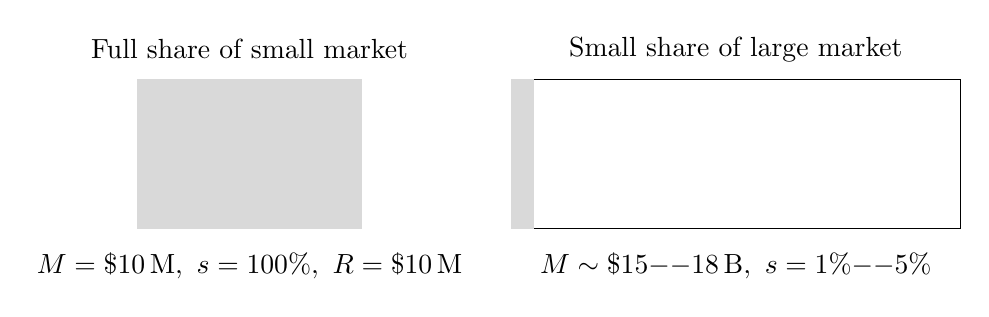
\begin{tikzpicture}[x=0.95cm,y=0.95cm]
\draw (0,0) rectangle (3,2);
\fill[black!15] (0,0) rectangle (3,2);
\node at (1.5,2.4) {Full share of small market};
\node at (1.5,-0.5) {$M=\$10\,\mathrm{M},\ s=100\%,\ R=\$10\,\mathrm{M}$};

\draw (5,0) rectangle (11,2);
\fill[black!15] (5,0) rectangle (5.3,2);
\node at (8,2.4) {Small share of large market};
\node at (8,-0.5) {$M\sim \$15\text{--}18\,\mathrm{B},\ s=1\%\text{--}5\%$};
\end{tikzpicture}
\end{figure}

The point of the figure is simple. The left case is complete control of a small rectangle. The right case is only a narrow strip of a much larger rectangle. Yet the right case may already dominate the left in dollars.

\paragraph{Worked example.}
The same interview also gives a small compounding model for service growth through referrals. The transcript says the first client paid
\begin{equation}
P_1 = \$5{,}000/\text{month},
\end{equation}
and that the work created
\begin{equation}
\Delta R_{\text{client}} = \$25\,\text{million}.
\end{equation}
That result generated three referrals. The monthly run rate therefore becomes
\begin{align}
N_{\text{referrals}} &= 3, \\
R_{\text{agency,monthly}} &= 4P_1 = 4\times \$5{,}000/\text{month} = \$20{,}000/\text{month}.
\end{align}
The arithmetic is elementary, but the lecture's point is not. Good work becomes its own acquisition channel.

\subsection{Question \& Answer}

Question: how can an operator start from zero and still buy a profitable business?

Answer: the lecture's answer is structural rather than exact in every number. One does not wait to save the entire purchase price in cash. One layers financing:
\begin{equation}
\text{Acquisition financing} = \text{seller note} + \text{SBA-backed bank financing}.
\end{equation}
The seller carries part of the note. The bank carries another part under SBA support. The acquired business is then improved through process discipline, technology, rankings, reviews, and lead generation. The transcript briefly mentions a down payment tied to profit, but the multiple is too noisy to stabilize. The safe point is the financing architecture itself.

After this interview the host makes an important meta-observation: once the mindset and skill set exist, wealth can be rebuilt from zero. That is the bridge to the final, rougher case.

\section{Transport, Place, and the Mentor Exit}

The final interview is shorter and less polished, but it performs an essential closing function. It returns the lecture from smoother business arithmetic to blunt field language: transport is durable, consistency matters, place matters, and if everything were lost one could build again.

The first claim is sectoral rather than numerical. The transport operator says that goods must still move, and so the industry remains difficult to replace. The second claim is procedural: consistency and repeated presence matter in sales and negotiation. But the sharpest mathematical content comes from the water example. The same water changes price when moved from one place to another. We may therefore write
\begin{equation}
P(w\mid L_1) \ne P(w\mid L_2),
\end{equation}
where \(w\) is the unchanged good and \(L_1,L_2\) are distinct market contexts.

\subsection{Question \& Answer}

Question: why can the same good have a different price in a different place without changing its physical substance?

Answer: because value is conditional on context, not on substance alone. Place contributes convenience, urgency, scarcity, social meaning, and the local structure of demand. The speaker gives the argument in compressed street language, but the logic is rigorous enough: price is a function of placement as well as object.

The lecture ends with a final mentorship rule. Once again the content is heuristic, but its role is clear:
\begin{equation}
\neg \text{mentor} \Rightarrow \text{directional drift}, \qquad
\text{mentor} + \text{observed bad moves} \Rightarrow \text{accelerated learning}.
\end{equation}
This last line gathers the chapter's earlier themes rather than replacing them. A mentor matters because he shortens the time required to see where the numbers, the people, and the hidden frictions really sit.

\section{Summary}

The lecture begins by promising scale and ends by localizing scale into mechanism. First, wealth is shown beginning not above zero but below it:
\[
W_0 = -\$20\,\text{million}.
\]
Then the chapter turns from biography to order: partners and banks are paid before the owner. From there it moves to commercial method: listen first, discover what counts as value, and only then speak about price. The host's own recap then turns that doctrine into customer feedback, and the salon founder resolves it into bathrooms, chairs, front desks, and investor alignment.

After the promotional interruption, the lecture reaches its cleanest arithmetic with Neil Patel. Revenue is separated from personal distributions, market size is separated from execution, and acquisition is separated from the fantasy that one must save the full purchase price in cash before acting. Finally, the transport interview compresses the entire lecture into a closing pair of rules: place changes price, and mentorship changes direction.

What remains is not a single theorem but a sequence of durable relations. Start even if the initial condition is negative. Preserve the trust of those who fund you. Listen before you price. Respect the force of tiny details. Do not confuse a small conquered market with a large opportunity. Understand that placement changes valuation. And remember that what the lecture finally admires is not merely having wealth, but knowing how to generate it again.